 \begin{solution}

\begin{enumerate}
\item {[8 points]} Let
\[
\psi_n(x) = \sqrt{2} \sin\left(n\pi x\right)
\]
for $n=1,2,\ldots$. The spectral method yields the series solution
\[
\tilde{u}(x,t)=\sum_{n=1}^\infty a_n(t)\psi_n(x)
\]
where
\begin{eqnarray*}
a_n(t)&=&\int_0^10\,dx e^{-n^2\pi^2t}+\int_0^te^{n^2\pi^2\left(s-t\right)}\int_0^1f(x,s)\psi_n(x)\,dx\,ds
\\
&=&\int_0^te^{n^2\pi^2\left(s-t\right)}\int_0^1f(x,s)\psi_n(x)\,dx\,ds.
\end{eqnarray*}
Now, for $n=1,2,3,\ldots$,
\begin{eqnarray*}
&&\int_0^1f(x,s)\psi_n(x)\,dx 
\\
&=& \sqrt{2}\left(\int_0^{1/2} f(x,s)\sin(n\pi x)\,dx+\int_{1/2}^1 f(x,s)\sin(n\pi x)\,dx\right)
\\
&=& 2\sqrt{2}\left(\int_0^{1/2} x\sin(n\pi x)\,dx+\int_{1/2}^1 (1-x)\sin(n\pi x)\,dx\right)
\\
&=&2\sqrt{2}\left(\left[-{1 \over n\pi}x\cos(n\pi x)\right]_0^{1/2}+{1 \over n\pi}\int_0^{1/2} \cos(n\pi x)\,dx+\left[-{1 \over n\pi}(1-x)\cos(n\pi x)\right]_{1/2}^1-{1 \over n\pi}\int_{1/2}^1 \cos(n\pi x)\,dx\right)
\\
&=&2\sqrt{2}\left(-{1 \over 2n\pi}\cos\left({n\pi \over 2}\right)+{1 \over n\pi}\int_0^{1/2} \cos(n\pi x)\,dx+{1 \over 2n\pi}\cos\left({n\pi \over 2}\right)-{1 \over n\pi}\int_{1/2}^1 \cos(n\pi x)\,dx\right)
\\
&=&\frac{2\sqrt{2}}{n\pi}\left(\int_0^{1/2} \cos(n\pi x)\,dx-\int_{1/2}^1 \cos(n\pi x)\,dx\right)
\\
&=&\frac{2\sqrt{2}}{n\pi}\left(\left[{1 \over n\pi}\sin(n\pi x)\right]_0^{1/2}-\left[{1 \over n\pi}\sin(n\pi x)\right]_{1/2}^1\right)
\\
&=&\frac{2\sqrt{2}}{n\pi}\left({1 \over n\pi}\sin\left(\frac{n\pi}{2}\right)+{1 \over n\pi}\sin\left(\frac{n\pi}{2}\right)\right)
\\
&=&\frac{4\sqrt{2}}{n^2\pi^2}\sin\left(\frac{n\pi}{2}\right).
\end{eqnarray*}
Consequently,
\begin{eqnarray*}
a_n(t)&=&\int_0^te^{n^2\pi^2\left(s-t\right)}\int_0^1f(x,s)\psi_n(x)\,dx\,ds
\\
&=&\frac{4\sqrt{2}}{n^2\pi^2}\sin\left(\frac{n\pi}{2}\right)\int_0^te^{n^2\pi^2\left(s-t\right)}\,ds
\\
&=&\frac{4\sqrt{2}}{n^2\pi^2}\sin\left(\frac{n\pi}{2}\right)\left[\frac{1}{n^2\pi^2}e^{n^2\pi^2\left(s-t\right)}\right]_{s=0}^{s=t}
\\
&=&\frac{4\sqrt{2}}{n^2\pi^2}\sin\left(\frac{n\pi}{2}\right)\left(\frac{1}{n^2\pi^2}-\frac{1}{n^2\pi^2}e^{-n^2\pi^2t}\right)
\\
&=&\frac{4\sqrt{2}}{n^4\pi^4}\sin\left(\frac{n\pi}{2}\right)\left(1-e^{-n^2\pi^2t}\right)
\end{eqnarray*}
and so
\[
\tilde{u}(x,t)=\sum_{n=1}^\infty\frac{8}{n^4\pi^4}\sin\left(\frac{n\pi}{2}\right)\left(1-e^{-n^2\pi^2t}\right)\sin(n\pi x).
\]

\item {[5 points]} The requested plot is below.

\begin{center}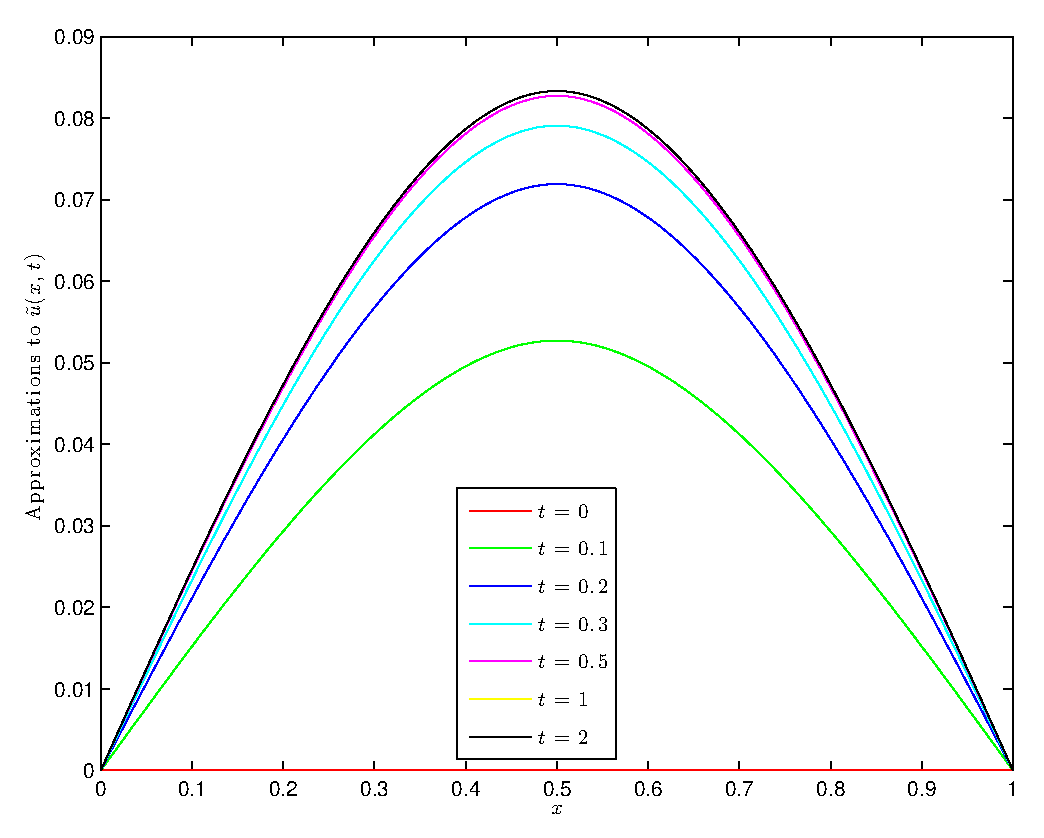
\includegraphics[scale=0.7]{hw38b.eps}\end{center}

The above plot was produced using the following MATLAB code.

\lstinputlisting{HW38b.m}

\item {[7 points]} Let
\[
w(x)=x
\]
so that
\[
w(0)=0
\]
and
\[
w(1)=1.
\]
Moreover, let $\hat{u}(x,t)$ be such that
\[
\hat{u}_t(x,t)-\hat{u}_{xx}(x,t) = f(x,t),\quad 0<x<1,\quad t>0;
\]
\[
\hat{u}(0,t) = \hat{u}(1,t) = 0,\quad t\ge0;
\]
and
\[
\hat{u}(x,0)=x^3-x,\quad 0<x<1.
\]
Then $u(x,t)=w(x)+\hat{u}(x,t)$ will be such that
\[
u_t(x,t)-u_{xx}(x,t)=\hat{u}_t(x,t)-w''(x)-\hat{u}_{xx}(x,t) = \hat{u}_t(x,t)-\hat{u}_{xx}(x,t) = f(x,t),\quad 0<x<1,\quad t>0;
\]
\[
u(0,t) = w(0) + \hat{u}(0,t) = 0+0 = 0,\quad t\ge0;
\]
\[
u(1,t) = w(1) + \hat{u}(1,t) = 1+0 = 1,\quad t\ge0;
\]
and
\[
u\left(x,0\right)=w(x)+\hat{u}(x,0)=x+x^3-x=x^3,\quad 0<x<1.
\]
The spectral method yields that
\[
\hat{u}(x,t)=\sum_{n=1}^\infty \hat{a}_n(t)\psi_n(x)
\]
where
\[
\hat{a}_n(t)=\int_0^1\left(x^3-x\right)\psi_n(x)\,dx e^{-n^2\pi^2t}+\int_0^te^{n^2\pi^2\left(s-t\right)}\int_0^1f(x,s)\psi_n(x)\,dx\,ds.
\]
Now, for $n=1,2,3,\ldots$,
\begin{eqnarray*}
\int_0^1\left(x^3-x\right)\psi_n(x)\,dx&=& \sqrt{2}\int_0^1 \left(x^3-x\right)\sin(n\pi x)\,dx
\\
&=&\sqrt{2}\left(\left[-{1 \over n\pi}\left(x^3-x\right)\cos(n\pi x)\right]_0^1+{1 \over n\pi}\int_0^1 \left(3x^2-1\right)\cos(n\pi x)\,dx\right)
\\
&=&{\sqrt{2} \over n\pi}\int_0^1 \left(3x^2-1\right)\cos(n\pi x)\,dx
\\
&=&{\sqrt{2} \over n\pi}\left(\left[{1 \over n\pi}\left(3x^2-1\right)\sin(n\pi x)\right]_0^1-{6 \over n\pi}\int_0^1 x\sin(n\pi x)\,dx\right)
\\
&=&-{6\sqrt{2} \over n^2\pi^2}\int_0^1 x\sin(n\pi x)\,dx
\\
&=&-{6\sqrt{2} \over n^2\pi^2}\left(\left[-{1 \over n\pi}x\cos(n\pi x)\right]_0^1+{1 \over n\pi}\int_0^1 \cos(n\pi x)\,dx\right)
\\
&=&-{6\sqrt{2} \over n^2\pi^2}\left(-{1 \over n\pi}\cos(n\pi)+{1 \over n\pi}\left[{1 \over n\pi} \sin(n\pi x)\right]_0^1\right)
\\
&=&{6\sqrt{2} \over n^3\pi^3}\cos(n\pi).
\end{eqnarray*}
Moreover, in part (a) we computed that, for $n=1,2,3,\ldots$,
\[
\int_0^te^{n^2\pi^2\left(s-t\right)}\int_0^1f(x,s)\psi_n(x)\,dx\,ds=\frac{4\sqrt{2}}{n^4\pi^4}\sin\left(\frac{n\pi}{2}\right)\left(1-e^{-n^2\pi^2t}\right).
\]
Hence,
\begin{eqnarray*}
\hat{a}_n(t)&=&\int_0^1\left(x^3-x\right)\psi_n(x)\,dx e^{-n^2\pi^2t}+\int_0^te^{n^2\pi^2\left(s-t\right)}\int_0^1f(x,s)\psi_n(x)\,dx\,ds
\\
&=&{6\sqrt{2} \over n^3\pi^3}\cos(n\pi)e^{-n^2\pi^2t}+\frac{4\sqrt{2}}{n^4\pi^4}\sin\left(\frac{n\pi}{2}\right)\left(1-e^{-n^2\pi^2t}\right)
\\
&=&{2\sqrt{2} \over n^3\pi^3}\left(\frac{2}{n\pi}\sin\left(\frac{n\pi}{2}\right)+\left(3\cos(n\pi)-\frac{2}{n\pi}\sin\left(\frac{n\pi}{2}\right)\right)e^{-n^2\pi^2t}\right)
\end{eqnarray*}
and so
\[
\hat{u}(x,t)=\sum_{n=1}^\infty {4 \over n^3\pi^3}\left(\frac{2}{n\pi}\sin\left(\frac{n\pi}{2}\right)+\left(3\cos(n\pi)-\frac{2}{n\pi}\sin\left(\frac{n\pi}{2}\right)\right)e^{-n^2\pi^2t}\right)\sin(n\pi x).
\]
Consequently,
\[
u(x,t)=x+\sum_{n=1}^\infty {4 \over n^3\pi^3}\left(\frac{2}{n\pi}\sin\left(\frac{n\pi}{2}\right)+\left(3\cos(n\pi)-\frac{2}{n\pi}\sin\left(\frac{n\pi}{2}\right)\right)e^{-n^2\pi^2t}\right)\sin(n\pi x).
\]

\item {[5 points]} The requested plot is below.

\begin{center}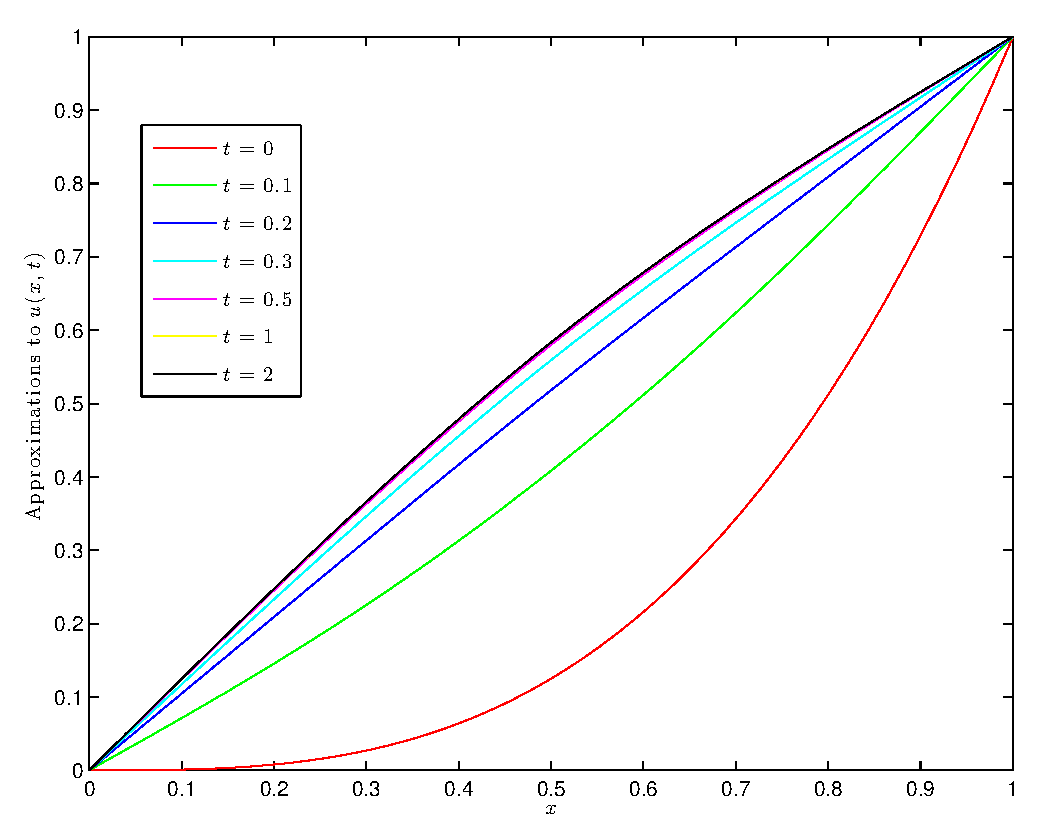
\includegraphics[scale=0.7]{hw38d.eps}\end{center}

The above plot was produced using the following MATLAB code.

\lstinputlisting{HW38d.m}

\end{enumerate}

\end{solution}